% Created by tikzDevice version 0.12.3.2 on 2022-02-15 17:02:35
% !TEX encoding = UTF-8 Unicode
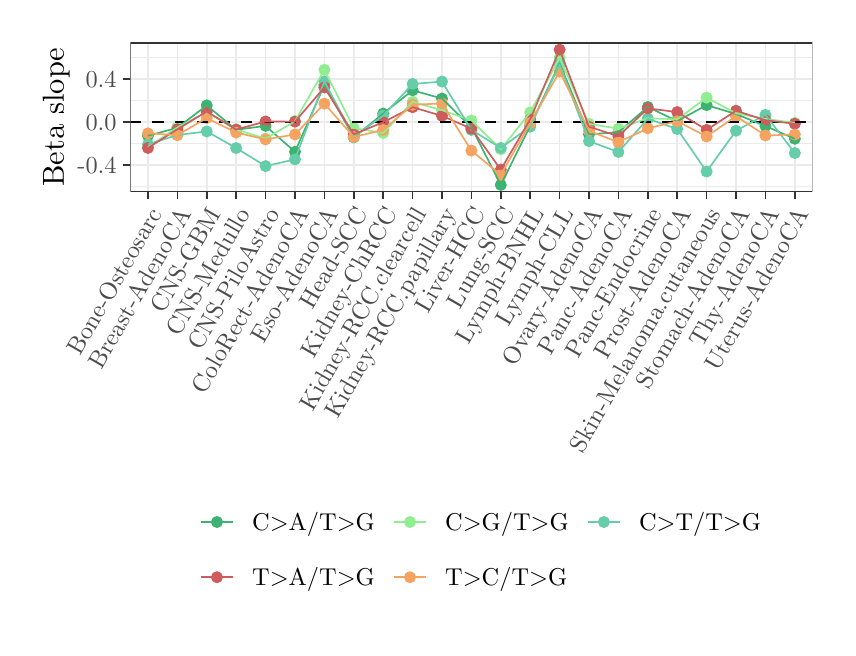
\begin{tikzpicture}[x=1pt,y=1pt]
\definecolor{fillColor}{RGB}{255,255,255}
\path[use as bounding box,fill=fillColor,fill opacity=0.00] (0,0) rectangle (289.08,216.81);
\begin{scope}
\path[clip] (  0.00,  0.00) rectangle (289.08,216.81);
\definecolor{drawColor}{RGB}{255,255,255}
\definecolor{fillColor}{RGB}{255,255,255}

\path[draw=drawColor,line width= 0.6pt,line join=round,line cap=round,fill=fillColor] (  0.00,  0.00) rectangle (289.08,216.81);
\end{scope}
\begin{scope}
\path[clip] ( 37.09,157.56) rectangle (283.58,211.31);
\definecolor{fillColor}{RGB}{255,255,255}

\path[fill=fillColor] ( 37.09,157.56) rectangle (283.58,211.31);
\definecolor{drawColor}{gray}{0.92}

\path[draw=drawColor,line width= 0.3pt,line join=round] ( 37.09,159.50) --
	(283.58,159.50);

\path[draw=drawColor,line width= 0.3pt,line join=round] ( 37.09,174.96) --
	(283.58,174.96);

\path[draw=drawColor,line width= 0.3pt,line join=round] ( 37.09,190.42) --
	(283.58,190.42);

\path[draw=drawColor,line width= 0.3pt,line join=round] ( 37.09,205.89) --
	(283.58,205.89);

\path[draw=drawColor,line width= 0.6pt,line join=round] ( 37.09,167.23) --
	(283.58,167.23);

\path[draw=drawColor,line width= 0.6pt,line join=round] ( 37.09,182.69) --
	(283.58,182.69);

\path[draw=drawColor,line width= 0.6pt,line join=round] ( 37.09,198.16) --
	(283.58,198.16);

\path[draw=drawColor,line width= 0.6pt,line join=round] ( 43.46,157.56) --
	( 43.46,211.31);

\path[draw=drawColor,line width= 0.6pt,line join=round] ( 54.09,157.56) --
	( 54.09,211.31);

\path[draw=drawColor,line width= 0.6pt,line join=round] ( 64.71,157.56) --
	( 64.71,211.31);

\path[draw=drawColor,line width= 0.6pt,line join=round] ( 75.34,157.56) --
	( 75.34,211.31);

\path[draw=drawColor,line width= 0.6pt,line join=round] ( 85.96,157.56) --
	( 85.96,211.31);

\path[draw=drawColor,line width= 0.6pt,line join=round] ( 96.59,157.56) --
	( 96.59,211.31);

\path[draw=drawColor,line width= 0.6pt,line join=round] (107.21,157.56) --
	(107.21,211.31);

\path[draw=drawColor,line width= 0.6pt,line join=round] (117.84,157.56) --
	(117.84,211.31);

\path[draw=drawColor,line width= 0.6pt,line join=round] (128.46,157.56) --
	(128.46,211.31);

\path[draw=drawColor,line width= 0.6pt,line join=round] (139.09,157.56) --
	(139.09,211.31);

\path[draw=drawColor,line width= 0.6pt,line join=round] (149.71,157.56) --
	(149.71,211.31);

\path[draw=drawColor,line width= 0.6pt,line join=round] (160.33,157.56) --
	(160.33,211.31);

\path[draw=drawColor,line width= 0.6pt,line join=round] (170.96,157.56) --
	(170.96,211.31);

\path[draw=drawColor,line width= 0.6pt,line join=round] (181.58,157.56) --
	(181.58,211.31);

\path[draw=drawColor,line width= 0.6pt,line join=round] (192.21,157.56) --
	(192.21,211.31);

\path[draw=drawColor,line width= 0.6pt,line join=round] (202.83,157.56) --
	(202.83,211.31);

\path[draw=drawColor,line width= 0.6pt,line join=round] (213.46,157.56) --
	(213.46,211.31);

\path[draw=drawColor,line width= 0.6pt,line join=round] (224.08,157.56) --
	(224.08,211.31);

\path[draw=drawColor,line width= 0.6pt,line join=round] (234.71,157.56) --
	(234.71,211.31);

\path[draw=drawColor,line width= 0.6pt,line join=round] (245.33,157.56) --
	(245.33,211.31);

\path[draw=drawColor,line width= 0.6pt,line join=round] (255.96,157.56) --
	(255.96,211.31);

\path[draw=drawColor,line width= 0.6pt,line join=round] (266.58,157.56) --
	(266.58,211.31);

\path[draw=drawColor,line width= 0.6pt,line join=round] (277.21,157.56) --
	(277.21,211.31);
\definecolor{drawColor}{RGB}{60,179,113}
\definecolor{fillColor}{RGB}{60,179,113}

\path[draw=drawColor,line width= 0.4pt,line join=round,line cap=round,fill=fillColor] ( 43.46,177.74) circle (  1.96);
\definecolor{drawColor}{RGB}{144,238,144}
\definecolor{fillColor}{RGB}{144,238,144}

\path[draw=drawColor,line width= 0.4pt,line join=round,line cap=round,fill=fillColor] ( 43.46,173.66) circle (  1.96);
\definecolor{drawColor}{RGB}{102,205,170}
\definecolor{fillColor}{RGB}{102,205,170}

\path[draw=drawColor,line width= 0.4pt,line join=round,line cap=round,fill=fillColor] ( 43.46,174.65) circle (  1.96);
\definecolor{drawColor}{RGB}{205,92,92}
\definecolor{fillColor}{RGB}{205,92,92}

\path[draw=drawColor,line width= 0.4pt,line join=round,line cap=round,fill=fillColor] ( 43.46,173.34) circle (  1.96);
\definecolor{drawColor}{RGB}{244,164,96}
\definecolor{fillColor}{RGB}{244,164,96}

\path[draw=drawColor,line width= 0.4pt,line join=round,line cap=round,fill=fillColor] ( 43.46,178.62) circle (  1.96);
\definecolor{drawColor}{RGB}{60,179,113}
\definecolor{fillColor}{RGB}{60,179,113}

\path[draw=drawColor,line width= 0.4pt,line join=round,line cap=round,fill=fillColor] ( 54.09,180.65) circle (  1.96);
\definecolor{drawColor}{RGB}{144,238,144}
\definecolor{fillColor}{RGB}{144,238,144}

\path[draw=drawColor,line width= 0.4pt,line join=round,line cap=round,fill=fillColor] ( 54.09,180.73) circle (  1.96);
\definecolor{drawColor}{RGB}{102,205,170}
\definecolor{fillColor}{RGB}{102,205,170}

\path[draw=drawColor,line width= 0.4pt,line join=round,line cap=round,fill=fillColor] ( 54.09,178.02) circle (  1.96);
\definecolor{drawColor}{RGB}{205,92,92}
\definecolor{fillColor}{RGB}{205,92,92}

\path[draw=drawColor,line width= 0.4pt,line join=round,line cap=round,fill=fillColor] ( 54.09,180.11) circle (  1.96);
\definecolor{drawColor}{RGB}{244,164,96}
\definecolor{fillColor}{RGB}{244,164,96}

\path[draw=drawColor,line width= 0.4pt,line join=round,line cap=round,fill=fillColor] ( 54.09,177.98) circle (  1.96);
\definecolor{drawColor}{RGB}{60,179,113}
\definecolor{fillColor}{RGB}{60,179,113}

\path[draw=drawColor,line width= 0.4pt,line join=round,line cap=round,fill=fillColor] ( 64.71,188.72) circle (  1.96);
\definecolor{drawColor}{RGB}{144,238,144}
\definecolor{fillColor}{RGB}{144,238,144}

\path[draw=drawColor,line width= 0.4pt,line join=round,line cap=round,fill=fillColor] ( 64.71,186.35) circle (  1.96);
\definecolor{drawColor}{RGB}{102,205,170}
\definecolor{fillColor}{RGB}{102,205,170}

\path[draw=drawColor,line width= 0.4pt,line join=round,line cap=round,fill=fillColor] ( 64.71,179.31) circle (  1.96);
\definecolor{drawColor}{RGB}{205,92,92}
\definecolor{fillColor}{RGB}{205,92,92}

\path[draw=drawColor,line width= 0.4pt,line join=round,line cap=round,fill=fillColor] ( 64.71,186.48) circle (  1.96);
\definecolor{drawColor}{RGB}{244,164,96}
\definecolor{fillColor}{RGB}{244,164,96}

\path[draw=drawColor,line width= 0.4pt,line join=round,line cap=round,fill=fillColor] ( 64.71,184.15) circle (  1.96);
\definecolor{drawColor}{RGB}{60,179,113}
\definecolor{fillColor}{RGB}{60,179,113}

\path[draw=drawColor,line width= 0.4pt,line join=round,line cap=round,fill=fillColor] ( 75.34,179.91) circle (  1.96);
\definecolor{drawColor}{RGB}{144,238,144}
\definecolor{fillColor}{RGB}{144,238,144}

\path[draw=drawColor,line width= 0.4pt,line join=round,line cap=round,fill=fillColor] ( 75.34,180.01) circle (  1.96);
\definecolor{drawColor}{RGB}{102,205,170}
\definecolor{fillColor}{RGB}{102,205,170}

\path[draw=drawColor,line width= 0.4pt,line join=round,line cap=round,fill=fillColor] ( 75.34,173.31) circle (  1.96);
\definecolor{drawColor}{RGB}{205,92,92}
\definecolor{fillColor}{RGB}{205,92,92}

\path[draw=drawColor,line width= 0.4pt,line join=round,line cap=round,fill=fillColor] ( 75.34,179.99) circle (  1.96);
\definecolor{drawColor}{RGB}{244,164,96}
\definecolor{fillColor}{RGB}{244,164,96}

\path[draw=drawColor,line width= 0.4pt,line join=round,line cap=round,fill=fillColor] ( 75.34,178.90) circle (  1.96);
\definecolor{drawColor}{RGB}{60,179,113}
\definecolor{fillColor}{RGB}{60,179,113}

\path[draw=drawColor,line width= 0.4pt,line join=round,line cap=round,fill=fillColor] ( 85.96,181.32) circle (  1.96);
\definecolor{drawColor}{RGB}{144,238,144}
\definecolor{fillColor}{RGB}{144,238,144}

\path[draw=drawColor,line width= 0.4pt,line join=round,line cap=round,fill=fillColor] ( 85.96,176.70) circle (  1.96);
\definecolor{drawColor}{RGB}{102,205,170}
\definecolor{fillColor}{RGB}{102,205,170}

\path[draw=drawColor,line width= 0.4pt,line join=round,line cap=round,fill=fillColor] ( 85.96,166.79) circle (  1.96);
\definecolor{drawColor}{RGB}{205,92,92}
\definecolor{fillColor}{RGB}{205,92,92}

\path[draw=drawColor,line width= 0.4pt,line join=round,line cap=round,fill=fillColor] ( 85.96,182.92) circle (  1.96);
\definecolor{drawColor}{RGB}{244,164,96}
\definecolor{fillColor}{RGB}{244,164,96}

\path[draw=drawColor,line width= 0.4pt,line join=round,line cap=round,fill=fillColor] ( 85.96,176.44) circle (  1.96);
\definecolor{drawColor}{RGB}{60,179,113}
\definecolor{fillColor}{RGB}{60,179,113}

\path[draw=drawColor,line width= 0.4pt,line join=round,line cap=round,fill=fillColor] ( 96.59,171.95) circle (  1.96);
\definecolor{drawColor}{RGB}{144,238,144}
\definecolor{fillColor}{RGB}{144,238,144}

\path[draw=drawColor,line width= 0.4pt,line join=round,line cap=round,fill=fillColor] ( 96.59,183.01) circle (  1.96);
\definecolor{drawColor}{RGB}{102,205,170}
\definecolor{fillColor}{RGB}{102,205,170}

\path[draw=drawColor,line width= 0.4pt,line join=round,line cap=round,fill=fillColor] ( 96.59,169.22) circle (  1.96);
\definecolor{drawColor}{RGB}{205,92,92}
\definecolor{fillColor}{RGB}{205,92,92}

\path[draw=drawColor,line width= 0.4pt,line join=round,line cap=round,fill=fillColor] ( 96.59,182.85) circle (  1.96);
\definecolor{drawColor}{RGB}{244,164,96}
\definecolor{fillColor}{RGB}{244,164,96}

\path[draw=drawColor,line width= 0.4pt,line join=round,line cap=round,fill=fillColor] ( 96.59,178.21) circle (  1.96);
\definecolor{drawColor}{RGB}{60,179,113}
\definecolor{fillColor}{RGB}{60,179,113}

\path[draw=drawColor,line width= 0.4pt,line join=round,line cap=round,fill=fillColor] (107.21,196.11) circle (  1.96);
\definecolor{drawColor}{RGB}{144,238,144}
\definecolor{fillColor}{RGB}{144,238,144}

\path[draw=drawColor,line width= 0.4pt,line join=round,line cap=round,fill=fillColor] (107.21,201.58) circle (  1.96);
\definecolor{drawColor}{RGB}{102,205,170}
\definecolor{fillColor}{RGB}{102,205,170}

\path[draw=drawColor,line width= 0.4pt,line join=round,line cap=round,fill=fillColor] (107.21,197.39) circle (  1.96);
\definecolor{drawColor}{RGB}{205,92,92}
\definecolor{fillColor}{RGB}{205,92,92}

\path[draw=drawColor,line width= 0.4pt,line join=round,line cap=round,fill=fillColor] (107.21,195.22) circle (  1.96);
\definecolor{drawColor}{RGB}{244,164,96}
\definecolor{fillColor}{RGB}{244,164,96}

\path[draw=drawColor,line width= 0.4pt,line join=round,line cap=round,fill=fillColor] (107.21,189.35) circle (  1.96);
\definecolor{drawColor}{RGB}{60,179,113}
\definecolor{fillColor}{RGB}{60,179,113}

\path[draw=drawColor,line width= 0.4pt,line join=round,line cap=round,fill=fillColor] (117.84,177.14) circle (  1.96);
\definecolor{drawColor}{RGB}{144,238,144}
\definecolor{fillColor}{RGB}{144,238,144}

\path[draw=drawColor,line width= 0.4pt,line join=round,line cap=round,fill=fillColor] (117.84,180.54) circle (  1.96);
\definecolor{drawColor}{RGB}{102,205,170}
\definecolor{fillColor}{RGB}{102,205,170}

\path[draw=drawColor,line width= 0.4pt,line join=round,line cap=round,fill=fillColor] (117.84,177.34) circle (  1.96);
\definecolor{drawColor}{RGB}{205,92,92}
\definecolor{fillColor}{RGB}{205,92,92}

\path[draw=drawColor,line width= 0.4pt,line join=round,line cap=round,fill=fillColor] (117.84,178.25) circle (  1.96);
\definecolor{drawColor}{RGB}{244,164,96}
\definecolor{fillColor}{RGB}{244,164,96}

\path[draw=drawColor,line width= 0.4pt,line join=round,line cap=round,fill=fillColor] (117.84,177.32) circle (  1.96);
\definecolor{drawColor}{RGB}{60,179,113}
\definecolor{fillColor}{RGB}{60,179,113}

\path[draw=drawColor,line width= 0.4pt,line join=round,line cap=round,fill=fillColor] (128.46,185.77) circle (  1.96);
\definecolor{drawColor}{RGB}{144,238,144}
\definecolor{fillColor}{RGB}{144,238,144}

\path[draw=drawColor,line width= 0.4pt,line join=round,line cap=round,fill=fillColor] (128.46,178.75) circle (  1.96);
\definecolor{drawColor}{RGB}{102,205,170}
\definecolor{fillColor}{RGB}{102,205,170}

\path[draw=drawColor,line width= 0.4pt,line join=round,line cap=round,fill=fillColor] (128.46,185.00) circle (  1.96);
\definecolor{drawColor}{RGB}{205,92,92}
\definecolor{fillColor}{RGB}{205,92,92}

\path[draw=drawColor,line width= 0.4pt,line join=round,line cap=round,fill=fillColor] (128.46,182.65) circle (  1.96);
\definecolor{drawColor}{RGB}{244,164,96}
\definecolor{fillColor}{RGB}{244,164,96}

\path[draw=drawColor,line width= 0.4pt,line join=round,line cap=round,fill=fillColor] (128.46,179.85) circle (  1.96);
\definecolor{drawColor}{RGB}{60,179,113}
\definecolor{fillColor}{RGB}{60,179,113}

\path[draw=drawColor,line width= 0.4pt,line join=round,line cap=round,fill=fillColor] (139.09,194.18) circle (  1.96);
\definecolor{drawColor}{RGB}{144,238,144}
\definecolor{fillColor}{RGB}{144,238,144}

\path[draw=drawColor,line width= 0.4pt,line join=round,line cap=round,fill=fillColor] (139.09,190.00) circle (  1.96);
\definecolor{drawColor}{RGB}{102,205,170}
\definecolor{fillColor}{RGB}{102,205,170}

\path[draw=drawColor,line width= 0.4pt,line join=round,line cap=round,fill=fillColor] (139.09,196.46) circle (  1.96);
\definecolor{drawColor}{RGB}{205,92,92}
\definecolor{fillColor}{RGB}{205,92,92}

\path[draw=drawColor,line width= 0.4pt,line join=round,line cap=round,fill=fillColor] (139.09,188.06) circle (  1.96);
\definecolor{drawColor}{RGB}{244,164,96}
\definecolor{fillColor}{RGB}{244,164,96}

\path[draw=drawColor,line width= 0.4pt,line join=round,line cap=round,fill=fillColor] (139.09,188.96) circle (  1.96);
\definecolor{drawColor}{RGB}{60,179,113}
\definecolor{fillColor}{RGB}{60,179,113}

\path[draw=drawColor,line width= 0.4pt,line join=round,line cap=round,fill=fillColor] (149.71,191.20) circle (  1.96);
\definecolor{drawColor}{RGB}{144,238,144}
\definecolor{fillColor}{RGB}{144,238,144}

\path[draw=drawColor,line width= 0.4pt,line join=round,line cap=round,fill=fillColor] (149.71,186.97) circle (  1.96);
\definecolor{drawColor}{RGB}{102,205,170}
\definecolor{fillColor}{RGB}{102,205,170}

\path[draw=drawColor,line width= 0.4pt,line join=round,line cap=round,fill=fillColor] (149.71,197.33) circle (  1.96);
\definecolor{drawColor}{RGB}{205,92,92}
\definecolor{fillColor}{RGB}{205,92,92}

\path[draw=drawColor,line width= 0.4pt,line join=round,line cap=round,fill=fillColor] (149.71,184.94) circle (  1.96);
\definecolor{drawColor}{RGB}{244,164,96}
\definecolor{fillColor}{RGB}{244,164,96}

\path[draw=drawColor,line width= 0.4pt,line join=round,line cap=round,fill=fillColor] (149.71,189.42) circle (  1.96);
\definecolor{drawColor}{RGB}{60,179,113}
\definecolor{fillColor}{RGB}{60,179,113}

\path[draw=drawColor,line width= 0.4pt,line join=round,line cap=round,fill=fillColor] (160.33,180.83) circle (  1.96);
\definecolor{drawColor}{RGB}{144,238,144}
\definecolor{fillColor}{RGB}{144,238,144}

\path[draw=drawColor,line width= 0.4pt,line join=round,line cap=round,fill=fillColor] (160.33,183.28) circle (  1.96);
\definecolor{drawColor}{RGB}{102,205,170}
\definecolor{fillColor}{RGB}{102,205,170}

\path[draw=drawColor,line width= 0.4pt,line join=round,line cap=round,fill=fillColor] (160.33,179.85) circle (  1.96);
\definecolor{drawColor}{RGB}{205,92,92}
\definecolor{fillColor}{RGB}{205,92,92}

\path[draw=drawColor,line width= 0.4pt,line join=round,line cap=round,fill=fillColor] (160.33,180.33) circle (  1.96);
\definecolor{drawColor}{RGB}{244,164,96}
\definecolor{fillColor}{RGB}{244,164,96}

\path[draw=drawColor,line width= 0.4pt,line join=round,line cap=round,fill=fillColor] (160.33,172.39) circle (  1.96);
\definecolor{drawColor}{RGB}{60,179,113}
\definecolor{fillColor}{RGB}{60,179,113}

\path[draw=drawColor,line width= 0.4pt,line join=round,line cap=round,fill=fillColor] (170.96,160.00) circle (  1.96);
\definecolor{drawColor}{RGB}{144,238,144}
\definecolor{fillColor}{RGB}{144,238,144}

\path[draw=drawColor,line width= 0.4pt,line join=round,line cap=round,fill=fillColor] (170.96,172.87) circle (  1.96);
\definecolor{drawColor}{RGB}{102,205,170}
\definecolor{fillColor}{RGB}{102,205,170}

\path[draw=drawColor,line width= 0.4pt,line join=round,line cap=round,fill=fillColor] (170.96,173.35) circle (  1.96);
\definecolor{drawColor}{RGB}{205,92,92}
\definecolor{fillColor}{RGB}{205,92,92}

\path[draw=drawColor,line width= 0.4pt,line join=round,line cap=round,fill=fillColor] (170.96,165.51) circle (  1.96);
\definecolor{drawColor}{RGB}{244,164,96}
\definecolor{fillColor}{RGB}{244,164,96}

\path[draw=drawColor,line width= 0.4pt,line join=round,line cap=round,fill=fillColor] (170.96,163.59) circle (  1.96);
\definecolor{drawColor}{RGB}{60,179,113}
\definecolor{fillColor}{RGB}{60,179,113}

\path[draw=drawColor,line width= 0.4pt,line join=round,line cap=round,fill=fillColor] (181.58,181.34) circle (  1.96);
\definecolor{drawColor}{RGB}{144,238,144}
\definecolor{fillColor}{RGB}{144,238,144}

\path[draw=drawColor,line width= 0.4pt,line join=round,line cap=round,fill=fillColor] (181.58,186.19) circle (  1.96);
\definecolor{drawColor}{RGB}{102,205,170}
\definecolor{fillColor}{RGB}{102,205,170}

\path[draw=drawColor,line width= 0.4pt,line join=round,line cap=round,fill=fillColor] (181.58,181.02) circle (  1.96);
\definecolor{drawColor}{RGB}{205,92,92}
\definecolor{fillColor}{RGB}{205,92,92}

\path[draw=drawColor,line width= 0.4pt,line join=round,line cap=round,fill=fillColor] (181.58,183.66) circle (  1.96);
\definecolor{drawColor}{RGB}{244,164,96}
\definecolor{fillColor}{RGB}{244,164,96}

\path[draw=drawColor,line width= 0.4pt,line join=round,line cap=round,fill=fillColor] (181.58,182.35) circle (  1.96);
\definecolor{drawColor}{RGB}{60,179,113}
\definecolor{fillColor}{RGB}{60,179,113}

\path[draw=drawColor,line width= 0.4pt,line join=round,line cap=round,fill=fillColor] (192.21,203.94) circle (  1.96);
\definecolor{drawColor}{RGB}{144,238,144}
\definecolor{fillColor}{RGB}{144,238,144}

\path[draw=drawColor,line width= 0.4pt,line join=round,line cap=round,fill=fillColor] (192.21,205.95) circle (  1.96);
\definecolor{drawColor}{RGB}{102,205,170}
\definecolor{fillColor}{RGB}{102,205,170}

\path[draw=drawColor,line width= 0.4pt,line join=round,line cap=round,fill=fillColor] (192.21,203.56) circle (  1.96);
\definecolor{drawColor}{RGB}{205,92,92}
\definecolor{fillColor}{RGB}{205,92,92}

\path[draw=drawColor,line width= 0.4pt,line join=round,line cap=round,fill=fillColor] (192.21,208.87) circle (  1.96);
\definecolor{drawColor}{RGB}{244,164,96}
\definecolor{fillColor}{RGB}{244,164,96}

\path[draw=drawColor,line width= 0.4pt,line join=round,line cap=round,fill=fillColor] (192.21,200.91) circle (  1.96);
\definecolor{drawColor}{RGB}{60,179,113}
\definecolor{fillColor}{RGB}{60,179,113}

\path[draw=drawColor,line width= 0.4pt,line join=round,line cap=round,fill=fillColor] (202.83,178.26) circle (  1.96);
\definecolor{drawColor}{RGB}{144,238,144}
\definecolor{fillColor}{RGB}{144,238,144}

\path[draw=drawColor,line width= 0.4pt,line join=round,line cap=round,fill=fillColor] (202.83,182.04) circle (  1.96);
\definecolor{drawColor}{RGB}{102,205,170}
\definecolor{fillColor}{RGB}{102,205,170}

\path[draw=drawColor,line width= 0.4pt,line join=round,line cap=round,fill=fillColor] (202.83,175.81) circle (  1.96);
\definecolor{drawColor}{RGB}{205,92,92}
\definecolor{fillColor}{RGB}{205,92,92}

\path[draw=drawColor,line width= 0.4pt,line join=round,line cap=round,fill=fillColor] (202.83,181.01) circle (  1.96);
\definecolor{drawColor}{RGB}{244,164,96}
\definecolor{fillColor}{RGB}{244,164,96}

\path[draw=drawColor,line width= 0.4pt,line join=round,line cap=round,fill=fillColor] (202.83,179.53) circle (  1.96);
\definecolor{drawColor}{RGB}{60,179,113}
\definecolor{fillColor}{RGB}{60,179,113}

\path[draw=drawColor,line width= 0.4pt,line join=round,line cap=round,fill=fillColor] (213.46,179.06) circle (  1.96);
\definecolor{drawColor}{RGB}{144,238,144}
\definecolor{fillColor}{RGB}{144,238,144}

\path[draw=drawColor,line width= 0.4pt,line join=round,line cap=round,fill=fillColor] (213.46,180.33) circle (  1.96);
\definecolor{drawColor}{RGB}{102,205,170}
\definecolor{fillColor}{RGB}{102,205,170}

\path[draw=drawColor,line width= 0.4pt,line join=round,line cap=round,fill=fillColor] (213.46,171.88) circle (  1.96);
\definecolor{drawColor}{RGB}{205,92,92}
\definecolor{fillColor}{RGB}{205,92,92}

\path[draw=drawColor,line width= 0.4pt,line join=round,line cap=round,fill=fillColor] (213.46,177.59) circle (  1.96);
\definecolor{drawColor}{RGB}{244,164,96}
\definecolor{fillColor}{RGB}{244,164,96}

\path[draw=drawColor,line width= 0.4pt,line join=round,line cap=round,fill=fillColor] (213.46,175.41) circle (  1.96);
\definecolor{drawColor}{RGB}{60,179,113}
\definecolor{fillColor}{RGB}{60,179,113}

\path[draw=drawColor,line width= 0.4pt,line join=round,line cap=round,fill=fillColor] (224.08,188.16) circle (  1.96);
\definecolor{drawColor}{RGB}{144,238,144}
\definecolor{fillColor}{RGB}{144,238,144}

\path[draw=drawColor,line width= 0.4pt,line join=round,line cap=round,fill=fillColor] (224.08,184.06) circle (  1.96);
\definecolor{drawColor}{RGB}{102,205,170}
\definecolor{fillColor}{RGB}{102,205,170}

\path[draw=drawColor,line width= 0.4pt,line join=round,line cap=round,fill=fillColor] (224.08,183.91) circle (  1.96);
\definecolor{drawColor}{RGB}{205,92,92}
\definecolor{fillColor}{RGB}{205,92,92}

\path[draw=drawColor,line width= 0.4pt,line join=round,line cap=round,fill=fillColor] (224.08,187.64) circle (  1.96);
\definecolor{drawColor}{RGB}{244,164,96}
\definecolor{fillColor}{RGB}{244,164,96}

\path[draw=drawColor,line width= 0.4pt,line join=round,line cap=round,fill=fillColor] (224.08,180.44) circle (  1.96);
\definecolor{drawColor}{RGB}{60,179,113}
\definecolor{fillColor}{RGB}{60,179,113}

\path[draw=drawColor,line width= 0.4pt,line join=round,line cap=round,fill=fillColor] (234.71,183.03) circle (  1.96);
\definecolor{drawColor}{RGB}{144,238,144}
\definecolor{fillColor}{RGB}{144,238,144}

\path[draw=drawColor,line width= 0.4pt,line join=round,line cap=round,fill=fillColor] (234.71,183.71) circle (  1.96);
\definecolor{drawColor}{RGB}{102,205,170}
\definecolor{fillColor}{RGB}{102,205,170}

\path[draw=drawColor,line width= 0.4pt,line join=round,line cap=round,fill=fillColor] (234.71,180.18) circle (  1.96);
\definecolor{drawColor}{RGB}{205,92,92}
\definecolor{fillColor}{RGB}{205,92,92}

\path[draw=drawColor,line width= 0.4pt,line join=round,line cap=round,fill=fillColor] (234.71,186.31) circle (  1.96);
\definecolor{drawColor}{RGB}{244,164,96}
\definecolor{fillColor}{RGB}{244,164,96}

\path[draw=drawColor,line width= 0.4pt,line join=round,line cap=round,fill=fillColor] (234.71,182.97) circle (  1.96);
\definecolor{drawColor}{RGB}{60,179,113}
\definecolor{fillColor}{RGB}{60,179,113}

\path[draw=drawColor,line width= 0.4pt,line join=round,line cap=round,fill=fillColor] (245.33,188.82) circle (  1.96);
\definecolor{drawColor}{RGB}{144,238,144}
\definecolor{fillColor}{RGB}{144,238,144}

\path[draw=drawColor,line width= 0.4pt,line join=round,line cap=round,fill=fillColor] (245.33,191.53) circle (  1.96);
\definecolor{drawColor}{RGB}{102,205,170}
\definecolor{fillColor}{RGB}{102,205,170}

\path[draw=drawColor,line width= 0.4pt,line join=round,line cap=round,fill=fillColor] (245.33,164.83) circle (  1.96);
\definecolor{drawColor}{RGB}{205,92,92}
\definecolor{fillColor}{RGB}{205,92,92}

\path[draw=drawColor,line width= 0.4pt,line join=round,line cap=round,fill=fillColor] (245.33,179.88) circle (  1.96);
\definecolor{drawColor}{RGB}{244,164,96}
\definecolor{fillColor}{RGB}{244,164,96}

\path[draw=drawColor,line width= 0.4pt,line join=round,line cap=round,fill=fillColor] (245.33,177.49) circle (  1.96);
\definecolor{drawColor}{RGB}{60,179,113}
\definecolor{fillColor}{RGB}{60,179,113}

\path[draw=drawColor,line width= 0.4pt,line join=round,line cap=round,fill=fillColor] (255.96,185.60) circle (  1.96);
\definecolor{drawColor}{RGB}{144,238,144}
\definecolor{fillColor}{RGB}{144,238,144}

\path[draw=drawColor,line width= 0.4pt,line join=round,line cap=round,fill=fillColor] (255.96,185.88) circle (  1.96);
\definecolor{drawColor}{RGB}{102,205,170}
\definecolor{fillColor}{RGB}{102,205,170}

\path[draw=drawColor,line width= 0.4pt,line join=round,line cap=round,fill=fillColor] (255.96,179.56) circle (  1.96);
\definecolor{drawColor}{RGB}{205,92,92}
\definecolor{fillColor}{RGB}{205,92,92}

\path[draw=drawColor,line width= 0.4pt,line join=round,line cap=round,fill=fillColor] (255.96,186.79) circle (  1.96);
\definecolor{drawColor}{RGB}{244,164,96}
\definecolor{fillColor}{RGB}{244,164,96}

\path[draw=drawColor,line width= 0.4pt,line join=round,line cap=round,fill=fillColor] (255.96,184.83) circle (  1.96);
\definecolor{drawColor}{RGB}{60,179,113}
\definecolor{fillColor}{RGB}{60,179,113}

\path[draw=drawColor,line width= 0.4pt,line join=round,line cap=round,fill=fillColor] (266.58,181.26) circle (  1.96);
\definecolor{drawColor}{RGB}{144,238,144}
\definecolor{fillColor}{RGB}{144,238,144}

\path[draw=drawColor,line width= 0.4pt,line join=round,line cap=round,fill=fillColor] (266.58,183.89) circle (  1.96);
\definecolor{drawColor}{RGB}{102,205,170}
\definecolor{fillColor}{RGB}{102,205,170}

\path[draw=drawColor,line width= 0.4pt,line join=round,line cap=round,fill=fillColor] (266.58,185.32) circle (  1.96);
\definecolor{drawColor}{RGB}{205,92,92}
\definecolor{fillColor}{RGB}{205,92,92}

\path[draw=drawColor,line width= 0.4pt,line join=round,line cap=round,fill=fillColor] (266.58,183.36) circle (  1.96);
\definecolor{drawColor}{RGB}{244,164,96}
\definecolor{fillColor}{RGB}{244,164,96}

\path[draw=drawColor,line width= 0.4pt,line join=round,line cap=round,fill=fillColor] (266.58,177.86) circle (  1.96);
\definecolor{drawColor}{RGB}{60,179,113}
\definecolor{fillColor}{RGB}{60,179,113}

\path[draw=drawColor,line width= 0.4pt,line join=round,line cap=round,fill=fillColor] (277.21,176.66) circle (  1.96);
\definecolor{drawColor}{RGB}{144,238,144}
\definecolor{fillColor}{RGB}{144,238,144}

\path[draw=drawColor,line width= 0.4pt,line join=round,line cap=round,fill=fillColor] (277.21,182.39) circle (  1.96);
\definecolor{drawColor}{RGB}{102,205,170}
\definecolor{fillColor}{RGB}{102,205,170}

\path[draw=drawColor,line width= 0.4pt,line join=round,line cap=round,fill=fillColor] (277.21,171.51) circle (  1.96);
\definecolor{drawColor}{RGB}{205,92,92}
\definecolor{fillColor}{RGB}{205,92,92}

\path[draw=drawColor,line width= 0.4pt,line join=round,line cap=round,fill=fillColor] (277.21,182.08) circle (  1.96);
\definecolor{drawColor}{RGB}{244,164,96}
\definecolor{fillColor}{RGB}{244,164,96}

\path[draw=drawColor,line width= 0.4pt,line join=round,line cap=round,fill=fillColor] (277.21,178.19) circle (  1.96);
\definecolor{drawColor}{RGB}{0,0,0}

\path[draw=drawColor,line width= 0.6pt,dash pattern=on 4pt off 4pt ,line join=round] ( 37.09,182.69) -- (283.58,182.69);
\definecolor{drawColor}{RGB}{60,179,113}

\path[draw=drawColor,line width= 0.6pt,line join=round] ( 43.46,177.74) --
	( 54.09,180.65) --
	( 64.71,188.72) --
	( 75.34,179.91) --
	( 85.96,181.32) --
	( 96.59,171.95) --
	(107.21,196.11) --
	(117.84,177.14) --
	(128.46,185.77) --
	(139.09,194.18) --
	(149.71,191.20) --
	(160.33,180.83) --
	(170.96,160.00) --
	(181.58,181.34) --
	(192.21,203.94) --
	(202.83,178.26) --
	(213.46,179.06) --
	(224.08,188.16) --
	(234.71,183.03) --
	(245.33,188.82) --
	(255.96,185.60) --
	(266.58,181.26) --
	(277.21,176.66);
\definecolor{drawColor}{RGB}{144,238,144}

\path[draw=drawColor,line width= 0.6pt,line join=round] ( 43.46,173.66) --
	( 54.09,180.73) --
	( 64.71,186.35) --
	( 75.34,180.01) --
	( 85.96,176.70) --
	( 96.59,183.01) --
	(107.21,201.58) --
	(117.84,180.54) --
	(128.46,178.75) --
	(139.09,190.00) --
	(149.71,186.97) --
	(160.33,183.28) --
	(170.96,172.87) --
	(181.58,186.19) --
	(192.21,205.95) --
	(202.83,182.04) --
	(213.46,180.33) --
	(224.08,184.06) --
	(234.71,183.71) --
	(245.33,191.53) --
	(255.96,185.88) --
	(266.58,183.89) --
	(277.21,182.39);
\definecolor{drawColor}{RGB}{102,205,170}

\path[draw=drawColor,line width= 0.6pt,line join=round] ( 43.46,174.65) --
	( 54.09,178.02) --
	( 64.71,179.31) --
	( 75.34,173.31) --
	( 85.96,166.79) --
	( 96.59,169.22) --
	(107.21,197.39) --
	(117.84,177.34) --
	(128.46,185.00) --
	(139.09,196.46) --
	(149.71,197.33) --
	(160.33,179.85) --
	(170.96,173.35) --
	(181.58,181.02) --
	(192.21,203.56) --
	(202.83,175.81) --
	(213.46,171.88) --
	(224.08,183.91) --
	(234.71,180.18) --
	(245.33,164.83) --
	(255.96,179.56) --
	(266.58,185.32) --
	(277.21,171.51);
\definecolor{drawColor}{RGB}{205,92,92}

\path[draw=drawColor,line width= 0.6pt,line join=round] ( 43.46,173.34) --
	( 54.09,180.11) --
	( 64.71,186.48) --
	( 75.34,179.99) --
	( 85.96,182.92) --
	( 96.59,182.85) --
	(107.21,195.22) --
	(117.84,178.25) --
	(128.46,182.65) --
	(139.09,188.06) --
	(149.71,184.94) --
	(160.33,180.33) --
	(170.96,165.51) --
	(181.58,183.66) --
	(192.21,208.87) --
	(202.83,181.01) --
	(213.46,177.59) --
	(224.08,187.64) --
	(234.71,186.31) --
	(245.33,179.88) --
	(255.96,186.79) --
	(266.58,183.36) --
	(277.21,182.08);
\definecolor{drawColor}{RGB}{244,164,96}

\path[draw=drawColor,line width= 0.6pt,line join=round] ( 43.46,178.62) --
	( 54.09,177.98) --
	( 64.71,184.15) --
	( 75.34,178.90) --
	( 85.96,176.44) --
	( 96.59,178.21) --
	(107.21,189.35) --
	(117.84,177.32) --
	(128.46,179.85) --
	(139.09,188.96) --
	(149.71,189.42) --
	(160.33,172.39) --
	(170.96,163.59) --
	(181.58,182.35) --
	(192.21,200.91) --
	(202.83,179.53) --
	(213.46,175.41) --
	(224.08,180.44) --
	(234.71,182.97) --
	(245.33,177.49) --
	(255.96,184.83) --
	(266.58,177.86) --
	(277.21,178.19);
\definecolor{drawColor}{gray}{0.20}

\path[draw=drawColor,line width= 0.6pt,line join=round,line cap=round] ( 37.09,157.56) rectangle (283.58,211.31);
\end{scope}
\begin{scope}
\path[clip] (  0.00,  0.00) rectangle (289.08,216.81);
\definecolor{drawColor}{gray}{0.30}

\node[text=drawColor,anchor=base east,inner sep=0pt, outer sep=0pt, scale=  0.88] at ( 32.14,164.20) {-0.4};

\node[text=drawColor,anchor=base east,inner sep=0pt, outer sep=0pt, scale=  0.88] at ( 32.14,179.66) {0.0};

\node[text=drawColor,anchor=base east,inner sep=0pt, outer sep=0pt, scale=  0.88] at ( 32.14,195.13) {0.4};
\end{scope}
\begin{scope}
\path[clip] (  0.00,  0.00) rectangle (289.08,216.81);
\definecolor{drawColor}{gray}{0.20}

\path[draw=drawColor,line width= 0.6pt,line join=round] ( 34.34,167.23) --
	( 37.09,167.23);

\path[draw=drawColor,line width= 0.6pt,line join=round] ( 34.34,182.69) --
	( 37.09,182.69);

\path[draw=drawColor,line width= 0.6pt,line join=round] ( 34.34,198.16) --
	( 37.09,198.16);
\end{scope}
\begin{scope}
\path[clip] (  0.00,  0.00) rectangle (289.08,216.81);
\definecolor{drawColor}{gray}{0.20}

\path[draw=drawColor,line width= 0.6pt,line join=round] ( 43.46,154.81) --
	( 43.46,157.56);

\path[draw=drawColor,line width= 0.6pt,line join=round] ( 54.09,154.81) --
	( 54.09,157.56);

\path[draw=drawColor,line width= 0.6pt,line join=round] ( 64.71,154.81) --
	( 64.71,157.56);

\path[draw=drawColor,line width= 0.6pt,line join=round] ( 75.34,154.81) --
	( 75.34,157.56);

\path[draw=drawColor,line width= 0.6pt,line join=round] ( 85.96,154.81) --
	( 85.96,157.56);

\path[draw=drawColor,line width= 0.6pt,line join=round] ( 96.59,154.81) --
	( 96.59,157.56);

\path[draw=drawColor,line width= 0.6pt,line join=round] (107.21,154.81) --
	(107.21,157.56);

\path[draw=drawColor,line width= 0.6pt,line join=round] (117.84,154.81) --
	(117.84,157.56);

\path[draw=drawColor,line width= 0.6pt,line join=round] (128.46,154.81) --
	(128.46,157.56);

\path[draw=drawColor,line width= 0.6pt,line join=round] (139.09,154.81) --
	(139.09,157.56);

\path[draw=drawColor,line width= 0.6pt,line join=round] (149.71,154.81) --
	(149.71,157.56);

\path[draw=drawColor,line width= 0.6pt,line join=round] (160.33,154.81) --
	(160.33,157.56);

\path[draw=drawColor,line width= 0.6pt,line join=round] (170.96,154.81) --
	(170.96,157.56);

\path[draw=drawColor,line width= 0.6pt,line join=round] (181.58,154.81) --
	(181.58,157.56);

\path[draw=drawColor,line width= 0.6pt,line join=round] (192.21,154.81) --
	(192.21,157.56);

\path[draw=drawColor,line width= 0.6pt,line join=round] (202.83,154.81) --
	(202.83,157.56);

\path[draw=drawColor,line width= 0.6pt,line join=round] (213.46,154.81) --
	(213.46,157.56);

\path[draw=drawColor,line width= 0.6pt,line join=round] (224.08,154.81) --
	(224.08,157.56);

\path[draw=drawColor,line width= 0.6pt,line join=round] (234.71,154.81) --
	(234.71,157.56);

\path[draw=drawColor,line width= 0.6pt,line join=round] (245.33,154.81) --
	(245.33,157.56);

\path[draw=drawColor,line width= 0.6pt,line join=round] (255.96,154.81) --
	(255.96,157.56);

\path[draw=drawColor,line width= 0.6pt,line join=round] (266.58,154.81) --
	(266.58,157.56);

\path[draw=drawColor,line width= 0.6pt,line join=round] (277.21,154.81) --
	(277.21,157.56);
\end{scope}
\begin{scope}
\path[clip] (  0.00,  0.00) rectangle (289.08,216.81);
\definecolor{drawColor}{gray}{0.30}

\node[text=drawColor,rotate= 60.00,anchor=base east,inner sep=0pt, outer sep=0pt, scale=  0.88] at ( 48.71,149.58) {Bone-Osteosarc};

\node[text=drawColor,rotate= 60.00,anchor=base east,inner sep=0pt, outer sep=0pt, scale=  0.88] at ( 59.34,149.58) {Breast-AdenoCA};

\node[text=drawColor,rotate= 60.00,anchor=base east,inner sep=0pt, outer sep=0pt, scale=  0.88] at ( 69.96,149.58) {CNS-GBM};

\node[text=drawColor,rotate= 60.00,anchor=base east,inner sep=0pt, outer sep=0pt, scale=  0.88] at ( 80.59,149.58) {CNS-Medullo};

\node[text=drawColor,rotate= 60.00,anchor=base east,inner sep=0pt, outer sep=0pt, scale=  0.88] at ( 91.21,149.58) {CNS-PiloAstro};

\node[text=drawColor,rotate= 60.00,anchor=base east,inner sep=0pt, outer sep=0pt, scale=  0.88] at (101.84,149.58) {ColoRect-AdenoCA};

\node[text=drawColor,rotate= 60.00,anchor=base east,inner sep=0pt, outer sep=0pt, scale=  0.88] at (112.46,149.58) {Eso-AdenoCA};

\node[text=drawColor,rotate= 60.00,anchor=base east,inner sep=0pt, outer sep=0pt, scale=  0.88] at (123.08,149.58) {Head-SCC};

\node[text=drawColor,rotate= 60.00,anchor=base east,inner sep=0pt, outer sep=0pt, scale=  0.88] at (133.71,149.58) {Kidney-ChRCC};

\node[text=drawColor,rotate= 60.00,anchor=base east,inner sep=0pt, outer sep=0pt, scale=  0.88] at (144.33,149.58) {Kidney-RCC.clearcell};

\node[text=drawColor,rotate= 60.00,anchor=base east,inner sep=0pt, outer sep=0pt, scale=  0.88] at (154.96,149.58) {Kidney-RCC.papillary};

\node[text=drawColor,rotate= 60.00,anchor=base east,inner sep=0pt, outer sep=0pt, scale=  0.88] at (165.58,149.58) {Liver-HCC};

\node[text=drawColor,rotate= 60.00,anchor=base east,inner sep=0pt, outer sep=0pt, scale=  0.88] at (176.21,149.58) {Lung-SCC};

\node[text=drawColor,rotate= 60.00,anchor=base east,inner sep=0pt, outer sep=0pt, scale=  0.88] at (186.83,149.58) {Lymph-BNHL};

\node[text=drawColor,rotate= 60.00,anchor=base east,inner sep=0pt, outer sep=0pt, scale=  0.88] at (197.46,149.58) {Lymph-CLL};

\node[text=drawColor,rotate= 60.00,anchor=base east,inner sep=0pt, outer sep=0pt, scale=  0.88] at (208.08,149.58) {Ovary-AdenoCA};

\node[text=drawColor,rotate= 60.00,anchor=base east,inner sep=0pt, outer sep=0pt, scale=  0.88] at (218.71,149.58) {Panc-AdenoCA};

\node[text=drawColor,rotate= 60.00,anchor=base east,inner sep=0pt, outer sep=0pt, scale=  0.88] at (229.33,149.58) {Panc-Endocrine};

\node[text=drawColor,rotate= 60.00,anchor=base east,inner sep=0pt, outer sep=0pt, scale=  0.88] at (239.96,149.58) {Prost-AdenoCA};

\node[text=drawColor,rotate= 60.00,anchor=base east,inner sep=0pt, outer sep=0pt, scale=  0.88] at (250.58,149.58) {Skin-Melanoma.cutaneous};

\node[text=drawColor,rotate= 60.00,anchor=base east,inner sep=0pt, outer sep=0pt, scale=  0.88] at (261.20,149.58) {Stomach-AdenoCA};

\node[text=drawColor,rotate= 60.00,anchor=base east,inner sep=0pt, outer sep=0pt, scale=  0.88] at (271.83,149.58) {Thy-AdenoCA};

\node[text=drawColor,rotate= 60.00,anchor=base east,inner sep=0pt, outer sep=0pt, scale=  0.88] at (282.45,149.58) {Uterus-AdenoCA};
\end{scope}
\begin{scope}
\path[clip] (  0.00,  0.00) rectangle (289.08,216.81);
\definecolor{drawColor}{RGB}{0,0,0}

\node[text=drawColor,rotate= 90.00,anchor=base,inner sep=0pt, outer sep=0pt, scale=  1.10] at ( 13.08,184.44) {Beta slope};
\end{scope}
\begin{scope}
\path[clip] (  0.00,  0.00) rectangle (289.08,216.81);
\definecolor{fillColor}{RGB}{255,255,255}

\path[fill=fillColor] ( 50.18,  5.50) rectangle (270.49, 50.91);
\end{scope}
\begin{scope}
\path[clip] (  0.00,  0.00) rectangle (289.08,216.81);
\definecolor{fillColor}{RGB}{255,255,255}

\path[fill=fillColor] ( 61.18, 30.95) rectangle ( 75.63, 45.41);
\end{scope}
\begin{scope}
\path[clip] (  0.00,  0.00) rectangle (289.08,216.81);
\definecolor{drawColor}{RGB}{60,179,113}
\definecolor{fillColor}{RGB}{60,179,113}

\path[draw=drawColor,line width= 0.4pt,line join=round,line cap=round,fill=fillColor] ( 68.40, 38.18) circle (  1.96);
\end{scope}
\begin{scope}
\path[clip] (  0.00,  0.00) rectangle (289.08,216.81);
\definecolor{drawColor}{RGB}{60,179,113}

\path[draw=drawColor,line width= 0.6pt,line join=round] ( 62.62, 38.18) -- ( 74.18, 38.18);
\end{scope}
\begin{scope}
\path[clip] (  0.00,  0.00) rectangle (289.08,216.81);
\definecolor{fillColor}{RGB}{255,255,255}

\path[fill=fillColor] (130.93, 30.95) rectangle (145.38, 45.41);
\end{scope}
\begin{scope}
\path[clip] (  0.00,  0.00) rectangle (289.08,216.81);
\definecolor{drawColor}{RGB}{144,238,144}
\definecolor{fillColor}{RGB}{144,238,144}

\path[draw=drawColor,line width= 0.4pt,line join=round,line cap=round,fill=fillColor] (138.15, 38.18) circle (  1.96);
\end{scope}
\begin{scope}
\path[clip] (  0.00,  0.00) rectangle (289.08,216.81);
\definecolor{drawColor}{RGB}{144,238,144}

\path[draw=drawColor,line width= 0.6pt,line join=round] (132.37, 38.18) -- (143.94, 38.18);
\end{scope}
\begin{scope}
\path[clip] (  0.00,  0.00) rectangle (289.08,216.81);
\definecolor{fillColor}{RGB}{255,255,255}

\path[fill=fillColor] (200.99, 30.95) rectangle (215.44, 45.41);
\end{scope}
\begin{scope}
\path[clip] (  0.00,  0.00) rectangle (289.08,216.81);
\definecolor{drawColor}{RGB}{102,205,170}
\definecolor{fillColor}{RGB}{102,205,170}

\path[draw=drawColor,line width= 0.4pt,line join=round,line cap=round,fill=fillColor] (208.21, 38.18) circle (  1.96);
\end{scope}
\begin{scope}
\path[clip] (  0.00,  0.00) rectangle (289.08,216.81);
\definecolor{drawColor}{RGB}{102,205,170}

\path[draw=drawColor,line width= 0.6pt,line join=round] (202.43, 38.18) -- (213.99, 38.18);
\end{scope}
\begin{scope}
\path[clip] (  0.00,  0.00) rectangle (289.08,216.81);
\definecolor{fillColor}{RGB}{255,255,255}

\path[fill=fillColor] ( 61.18, 11.00) rectangle ( 75.63, 25.45);
\end{scope}
\begin{scope}
\path[clip] (  0.00,  0.00) rectangle (289.08,216.81);
\definecolor{drawColor}{RGB}{205,92,92}
\definecolor{fillColor}{RGB}{205,92,92}

\path[draw=drawColor,line width= 0.4pt,line join=round,line cap=round,fill=fillColor] ( 68.40, 18.23) circle (  1.96);
\end{scope}
\begin{scope}
\path[clip] (  0.00,  0.00) rectangle (289.08,216.81);
\definecolor{drawColor}{RGB}{205,92,92}

\path[draw=drawColor,line width= 0.6pt,line join=round] ( 62.62, 18.23) -- ( 74.18, 18.23);
\end{scope}
\begin{scope}
\path[clip] (  0.00,  0.00) rectangle (289.08,216.81);
\definecolor{fillColor}{RGB}{255,255,255}

\path[fill=fillColor] (130.93, 11.00) rectangle (145.38, 25.45);
\end{scope}
\begin{scope}
\path[clip] (  0.00,  0.00) rectangle (289.08,216.81);
\definecolor{drawColor}{RGB}{244,164,96}
\definecolor{fillColor}{RGB}{244,164,96}

\path[draw=drawColor,line width= 0.4pt,line join=round,line cap=round,fill=fillColor] (138.15, 18.23) circle (  1.96);
\end{scope}
\begin{scope}
\path[clip] (  0.00,  0.00) rectangle (289.08,216.81);
\definecolor{drawColor}{RGB}{244,164,96}

\path[draw=drawColor,line width= 0.6pt,line join=round] (132.37, 18.23) -- (143.94, 18.23);
\end{scope}
\begin{scope}
\path[clip] (  0.00,  0.00) rectangle (289.08,216.81);
\definecolor{drawColor}{RGB}{0,0,0}

\node[text=drawColor,anchor=base west,inner sep=0pt, outer sep=0pt, scale=  0.88] at ( 81.13, 35.15) {C$>$A/T$>$G};
\end{scope}
\begin{scope}
\path[clip] (  0.00,  0.00) rectangle (289.08,216.81);
\definecolor{drawColor}{RGB}{0,0,0}

\node[text=drawColor,anchor=base west,inner sep=0pt, outer sep=0pt, scale=  0.88] at (150.88, 35.15) {C$>$G/T$>$G};
\end{scope}
\begin{scope}
\path[clip] (  0.00,  0.00) rectangle (289.08,216.81);
\definecolor{drawColor}{RGB}{0,0,0}

\node[text=drawColor,anchor=base west,inner sep=0pt, outer sep=0pt, scale=  0.88] at (220.94, 35.15) {C$>$T/T$>$G};
\end{scope}
\begin{scope}
\path[clip] (  0.00,  0.00) rectangle (289.08,216.81);
\definecolor{drawColor}{RGB}{0,0,0}

\node[text=drawColor,anchor=base west,inner sep=0pt, outer sep=0pt, scale=  0.88] at ( 81.13, 15.20) {T$>$A/T$>$G};
\end{scope}
\begin{scope}
\path[clip] (  0.00,  0.00) rectangle (289.08,216.81);
\definecolor{drawColor}{RGB}{0,0,0}

\node[text=drawColor,anchor=base west,inner sep=0pt, outer sep=0pt, scale=  0.88] at (150.88, 15.20) {T$>$C/T$>$G};
\end{scope}
\end{tikzpicture}
